%thesis.tex 
%Model LaTeX file for Ph.D. thesis at the 
%School of Mathematics, University of Edinburgh

\title{Fairness in Transfer Learning for Natural Language Processing}
\author{Seraphina Goldfarb-Tarrant}
\date{2023}

\documentclass[phd,ilcc,oneside,leftchapter,parskip]{infthesis}

\usepackage[T2A,T1]{fontenc}
\usepackage[utf8x]{inputenc}

\usepackage[english]{babel}

\usepackage{natbib}

% \usepackage{biblatex}
% \addbibresource{biblatex_bib.bib}

\usepackage{latexsym}
\usepackage{graphicx}
\usepackage{amsmath}
\usepackage{wrapfig}
\usepackage{times}

\usepackage[dvipsnames]{xcolor}

\usepackage{subcaption}
\usepackage{mwe}
\usepackage{booktabs} % Top and bottom rules for tables
\usepackage{svrsymbols}

\usepackage{tikz-dependency}
\usepackage{tikz-qtree}
\usepackage{paralist}
\usepackage{tikz}
\usetikzlibrary{shapes,arrows,positioning}
\usetikzlibrary{matrix}
\usepackage{etoolbox}
\usepackage{bm}
\usepackage{amssymb}
\usepackage{amsfonts}
\usepackage{amsmath}
\usepackage{csquotes}
\usepackage{verbatim}
% \usepackage{todonotes}

\usepackage{epigraph}
\setlength{\epigraphwidth}{0.7\textwidth} 

\usepackage[final]{pdfpages}

\usepackage{url}
\usepackage{hyperref}
\usepackage{cleveref}
\urlstyle{rm}
\definecolor{revcolor}{rgb}{0.81, 0.09, 0.13}
\definecolor{darkblue}{rgb}{0.2, 0.2, 0.6}


\usepackage[left, mathlines]{lineno}
\renewcommand\linenumberfont{\normalfont\bfseries\small\color{lightgray}}

\hypersetup{
    colorlinks,
    citecolor=darkblue,
    filecolor=black,
    linkcolor=darkblue,
    urlcolor=darkblue
}

% \usepackage{lsubfiles}

\newcommand{\sgtcomment}[1]{\textcolor{blue}{[ST: #1]}}

\newcommand{\E}{\mathbb{E}}


\abstract{Natural Language Processing (NLP) systems have come to permeate so many areas of daily life that it is difficult to live a day without having one or many experiences mediated by an NLP system. These systems bring with them many promises -- more accessible information in more languages, real-time content moderation, more data-driven decision making, intuitive access to information via Q&A and chat interfaces.
%and scale and efficiency at low costs. 
But there is a dark side to these promises, for the past decade of research has shown that NLP systems can contain social biases and deploying them can incur serious social costs. Each of these promises has been found to have unintended consequences: racially charged errors and rampant gender stereotyping in language translation, censorship of minority voices and dialects, Human Resource systems that discriminate based on demographic data, a proliferation of toxic generated text and misinformation, and many subtler issues. 

Yet despite these consequences, and the proliferation of bias research attempting to correct them, NLP systems have not improved very much. There are a few reasons for this. First, measuring bias is difficult; there are not standardised methods of measurement, and much research relies on one-off methods that are often insufficiently careful and thoroughly tested. Thus many works have contradictory results that cannot be reconciled, because of minor differences or assumptions in their metrics. Without thorough testing, these metrics can even mislead and give the illusion of progress. Second, much research adopts an overly simplistic view of the causes and mediators of bias in a system. NLP systems have multiple components and stages of training, and many works test fairness at only one stage. They do not study how different parts of the system interact, and how fairness changes during this process. So it is unclear whether these isolated results will hold in the full complex system. Here, we address both of these shortcomings. We conduct a detailed analysis of fairness metrics applied to upstream language models (models that will be used in a downstream task in transfer learning). We find that a) the most commonly used upstream fairness metric is not predictive of downstream fairness, such that it should not be used but that b) information theoretic probing is a good alternative to these existing fairness metrics, as we find it is both predictive of downstream bias and robust to different modelling choices.   %illuminating the inconsistencies in a number of common metrics, and making recommendations to improve their utility. 
We then use our findings to track how unfairness, having entered a system, persists and travels throughout it. We track how fairness issues travel between tasks (from language modelling to classification) in monolingual transfer learning, and between languages, in multilingual transfer learning. We find that multilingual transfer learning often exacerbates fairness problems and should be used with care, whereas monolingual transfer learning generally improves fairness. Finally, we track how fairness travels between source documents and retrieved answers to questions, in fact-based generative systems. Here we find that, though retrieval systems strongly represent demographic data such as gender, bias in retrieval question answering benchmarks does not come from the model representations, but from the queries or the corpora. We reach all of our findings only by looking at the entire transfer learning system as a whole, and we hope that this encourages other researchers to do the same. We hope that our results can guide future fairness research to be more consistent between works, better predictive of real world fairness outcomes, and better able to prevent unfairness from propagating between different parts of a system. 
}

\begin{document}

%% First, the preliminary pages
\begin{preliminary}

%% This creates the title page
\maketitle


\begin{laysummary}
Laysummary
\end{laysummary}

% Acknowledgements
\begin{acknowledgements}
ACK


\end{acknowledgements}


%% Next we need to have the declaration.
\standarddeclaration

\dedication{}

%% Finally, a dedication (this is optional -- uncomment the following line if
%% you want one).
% \dedication{To my mum
%% Create the table of contents
\tableofcontents

%% If you want a list of figures or tables, uncomment the appropriate line(s)
% \listoffigures
% \listoftables

\end{preliminary}
%\linenumbers

%!TEX root = ../thesis.tex
\chapter{Introduction} 
\label{chapter:introduction}
In the past decade, Natural Language Processing (NLP) systems have come to saturate everyday life. NLP has expanded from being used to translate webpages and recommend new videos to having inescapable reach. It is now also used to moderate social media content \citep{ofcom_content_mod}, where all posts are filtered through an NLP system that judges them as hateful/not-hateful, acceptable/not-acceptable, and either removes or suppresses the sharing of posts that fail this check. NLP is used to generate answers to any user questions about any topic \citep{rajpurkar-etal-2016-squad, rajpurkar-etal-2018-know}, by sifting through millions of documents and determining which ones are relevant and worth knowing about and presenting those, discarding others. It is used to  track public opinion about products or politicians \citep{peoples-2020-modeling}, by analysing the sentiment of all of the information said about them online. NLP is used to sort and filter resumes for potential new workers \citep{parasurama-sedoc-2022-gendered}, by comparing each new resume to previous successful hires for a job, and flagging which ones to send to a phone-screen and which ones to reject. It is also used to later fire those same workers \citep{forbes_hiring}, by reading data about their productivity and predicting who shouldn't make the cut. These examples are a small set of the myriad applications that use NLP today, chosen as the areas the are directly relevant to the research in this thesis. There are so many more; most people in the UK and US come into contact with NLP or AI multiple times daily, though many of them are not aware of it \citep{kennedy2023public}.

This increase in scope and usage of NLP systems comes with many promises of efficiency, cost reduction, and even social good. For all of the uses above, there are bright promises. NLP for content moderation on social media can reduce hatespeech and aggression online, which has reached a volume and velocity that is completely unmanageable for human moderators. When left unchecked, it is linked to amplification of violence in the real world. NLP for retrieval and question answering can enable greater and easier access to information, a necessary step in searching and organising the vast quantities of digital information and democratising information access. NLP as sentiment analysis of public opinion can enable direct and inexpensive democratic feedback for companies or policies; direct feedback that might otherwise be too logistically challenging and expensive to gather. NLP in hiring systems could enable processing more applications, which could give a broader segment of the population a chance, and create systems that are less dependent on `who you know' and on the instincts of a few HR representatives tasked with reading through a resume slush pile.

But this territorial expansion introduces many new harms that diminish these promises.  
The often referenced promise of mathematical objectivity---freeing us from human subjectivity, inconsistency, and biases---has proven to be mythical. 
At best, NLP systems learn and propagate these same biases, but with a veneer of objectivity that fosters over-reliance \citep{oneil2016weapons} and reduces accountability and recourse when data is incorrect and decisions go wrong. 

A large and growing body of work analysing NLP systems has shown that they do not behave similarly and work equally well for different genders, races, nationalities, and other demographic groups. This disparate performance across demographics is the standard definition of \textbf{fairness}, which we use throughout this thesis: these systems are not \textbf{fair}. 
So given that NLP systems, and the data, models, and optimisation and evaluation metrics they are composed of are \textit{not} inherently fair, we must analyse the ways they are not, so we know what to expect and can mitigate where possible. When NLP systems are not fair, companies and organisations using them (and people subjected to their outputs) are worse off than before automation systems, since this flawed system has now been scaled. An individual Human Resources manager may have flaws and biases, but they work for only one or a few companies and have time to read only so many resumes in a day. Some resumes will be sent to a different person, who may have different biases, preventing the inequities of the first person's views from being complete and consistent over a wide swath of potential jobs. When a flawed and biased NLP HR system is scaled, it does not sleep, get tired, or clock-off and can process as many thousands of resumes as time and compute allows. The same system is used by many companies. The very variability of human behaviour, and the inconsistencies in human decisionmaking that are often considered undesirable, limit the possible scope of each individual's (or even each company or organisation's) biases. This lack of scaling of humans is an accidental safeguard. An NLP system, in contrast, replicates the same biases to an unlimited extent, and whatever unfortunate minorities it is biased against will experience more widespread discrimination. This is the situation of the present day, and sets the scene for this research.

The research world noticed this, eventually. Fairness problems in NLP started to become well-known in the NLP community in 2016, as NLP itself began to directly touch more lives and have more impact \citep{hovy-spruit-2016-social}. Attention in the research world, and the public, has grown exponentially since\footnote{\url{https://fairmlclass.github.io/1.html\#/4}}. By the time of writing, major conferences now have a dedicated track for fairness research\footnote{\url{https://aclrollingreview.org/cfp}}, encourage papers to self-declare potential hazards\footnote{Section A2 in \url{https://aclrollingreview.org/responsibleNLPresearch/}, and section 1c in \url{https://neurips.cc/Conferences/2021/PaperInformation/PaperChecklist}}, and have an ethics committee appointed to review potential fairness problems in any work\footnote{\url{https://www.aclweb.org/adminwiki/index.php?title=Formation_of_the_ACL_Ethics_Committee}}. Yet despite all the attention and effort expended on fairness in NLP, we as a community have made only such a small dent in known problems as to now be aware of the magnitude of still unaddressed fairness problems. Both discovering and addressing fairness problems in an NLP system remains extremely challenging. 

There are a couple of reasons for this challenge, which have prevented the community from making a larger dent. One of the most salient ones is that NLP systems today are complex; they involve multiple stages of model training, as is the case with Transfer Learning (discussed and defined in \S\ref{sec:bg_transfer_learning}). How to measure and mitigate unfairness in a multi-part NLP system is not clear, and systems are now always multi-part. How does a measurement or mitigation at one stage relate to the other stages? What can be trusted to hold across stages? This thesis attempts to take a step towards remedying this. It asserts, throughout each of the sections, that you cannot study just one part of an NLP system in isolation, without first understanding how it affects the other parts. 

There is real difficulty in even defining unfairness, and a substantial percentage of fairness papers neglect to define it at all \citep{blodgett-etal-2020-language, goldfarb-tarrant-etal-2023-prompt}. There are multiple ways that a system can be unfair. NLP systems are often not \textbf{allocationally fair}; they and have different accuracies and rates of false positives and false negatives for different demographics. A example such situation is when a toxicity detection system has much higher rates of false positives for text that is actually neutral or positive but contains terms about race, religion, or sexual orientation. In such as case, a sentence like \textit{I am a gay man} can be flagged as toxic and censored, as was the case with Google's toxicity detection system in 2018 \citep{Dixon2018MeasuringAM}. NLP systems are also often not \textbf{representationally fair}; they reproduce and propagate negative stereotypes for minoritised demographics \citep{crawford_keynote}. For example, prominent generation systems will disproportionately describe women as taking carer roles, and portray racial minorities as criminals \citep{sheng-etal-2019-woman}. 

There is not even a consensus on how best to measure each type of unfairness. Most metrics used to measure fairness are ad-hoc and have not been standardised or analysed for \textbf{predictive validity}---their ability to predict actual fairness problems that will occur--or \textbf{concurrent validity}---their agreement with other metrics in use. If you cannot measure something, `your knowledge is of a meagre and unsatisfactory kind' \citep{kelvin1891popular} and you cannot know whether any improvements you make actually worked. So we begin by making some progress towards assessing predictive and concurrent validity of fairness metrics in Part~\ref{part:measurement}.  

Another challenge is that fairness issues can appear at almost any stage of building an NLP system \citep{suresh2021framework}, and as mentioned, the relationship between the stages is poorly understood. NLP papers commonly claim that `model biases reflect biases in data they were trained on'\footnote{This refrain is ubiquitous, and is apparently even the rationale that ChatGPT gives: \textit{Yes, language models can have biases, because the training data reflects the biases present in society from which that data was collected.} as reported in \url{https://news.mit.edu/2023/large-language-models-are-biased-can-logic-help-save-them-0303}} 
but this is such a gross oversimplification as to be both unhelpful and misleading. It glosses over questions such as: \textit{how did the biases get into the data? Do imbalances in labels over different sensitive groups count, or do only stereotypes count?} And it glosses over all the other causes, of which there are seven high level kinds in \citet{suresh2021framework}, and some additional in other works \citep{mehrabi_survey}. I expect the prevalence of this statement is a way of shirking responsibility. If it is the data's fault for being biased, and society's fault for creating biased data, then it is not the fault of the engineer or company for creating a biased model. It's just the world we live in. 

But it is not the world we live in. It is the world we are making. All choices in the process of training an NLP model can affect the resulting bias. A resume filtering system can be trained on data in which humans made racist or sexist decisions -- say in the past they didn't hire non-men, or non-white, or only hired young people or people who went to certain schools. This is \textbf{historical} bias, and that bias in the training data will not only persist, but be amplified, an effect which is much less frequently discussed but is common \citep{zhao-etal-2017-men, jia-etal-2020-mitigating, cabello-etal-2023-evaluating, pmlr-v80-hashimoto18a}. 
%This already weakens the ability to shirk responsibility for a system that not only reflects existing societal biases, but increases them . 
Then this system, which is already dubiously `only reflecting training data' will scale, with the authority of an objective AI system behind it. This happened with Amazon's attempt at an AI for Human Resources, which would not hire women at all because, historically, Amazon had not hired very many of them.\footnote{\url{https://www.reuters.com/article/us-amazon-com-jobs-automation-insight-idUSKCN1MK08G}.} There are also \textbf{sampling}, aka \textbf{representation}, biases. For instance, a content moderation and toxicity detection system can be unfamiliar with non-prestige dialects and censor them incorrectly, as happened when tweets in African-American Vernacular English (AAVE) were incorrectly flagged as toxic speech \citep{sap-etal-2019-risk}. Even though AAVE is common in the \textit{world}, it was not well-represented in data the model has seen. So even within dataset biases, there are multiple kinds with different reasons behind them. There are other sources beyond dataset biases. The above example of historical bias in hiring is actually an example of another type of bias as well, \textbf{measurement} bias. This NLP resume filtering system uses labelled data for supervised learning (as is quite common) where the labels are a proxy for the task that is to be learnt -- e.g. \textit{was previously hired based on this resume} is a proxy for \textit{was suitable for the job}. That label can be a better or worse proxy for the desired task. This gap between the thing being measured and the unmeasurable quantity of interest is \textbf{measurement} bias. These are only a few of the many ways that unfairness can enter a system, selected as examples as they are the types that I spend the most time examining below. There are more subtle ways that can make mitigation even more challenging, which I discuss in Part~\ref{chapter:background}.

% Remining things are aggregation (example from hardt) and evaluation (maybe example from my reality check paper) and also learning (the metric being optimised). 

%Fairness issues can arise also in fitting the same function to multiple groups that require different functions (aggregation bias) and in the metric used to evaluate (evaluation bias) \citep{hardt2016equality}.


%it has become a vital responsibilty for us as researchers to examine our models, algorithms, and data as to their behaviour for different demographic groups. Do they behave similarly and work equally well for different genders, different races, different nationalities? We need to know this information to ensure that the systems we build innovate, and improve society, rather than accelerating marginalisation and societal divisions and isolation. 

%These are the ways that unfairness can enter a system. 

%PICK UP HERE -- connect to the issues of *scaling* and of *not knowing how something gets into the system. Might need to connect transfer learning to it more smoothly -- since transfer learning is responsible for scale, and basically introduces a new source of all of these types of biases that is unexplored (a second set of data and of sampling and of measurement blah blah). It is also now the dominant paradigm (scale) that has been underexplored. And we want to know if these systems are better or worse than systems before using them, and we also want to pinpoint the source to enable us to mitigate it -- if we performed mitigation at the wrong stage it might not work

An NLP system can contain one, many, or all of these sources of bias, and this bias can enter in via the data collection, dataset splits, learning objective, model architecture, model deployment choices (such as decoding hyperparameters or classifier thresholds). And most of these choices are now made \textit{twice} or more. Current scale in NLP is driven by \textbf{transfer learning}, where a model is trained on high resource task(s) or language(s) (e.g. unstructured web crawl text) and then ported to a lower resourced one (e.g. any supervised task requiring labels, like sentiment analysis) -- not necessarily objectively \textit{low resource}, but relatively lower resourced, i.e. with less data than the dominant task or language being used for transfer. 
%Within a language, this is usually done with a language model pre-trained on large scale web text and then applied to a supervised learning task requiring labelled data. Between languages, this is usually done between English and another language with less or no labelled data. 
It was already difficult to pinpoint where biases enter a system, and with transfer learning most systems are composed of multiple sets of training data, multiple objectives, multiple measurements. 
%The little work on existing multi-part systems shows that individually fair components are not necessarily fair under composition \citep{dwork2018group}

Transfer learning is now the dominant paradigm in NLP, but previous to the work in this thesis, fairness research considered only one of the two stages: the pre-training or the fine-tuning stage. If a language model that will later be used in our example resume filtering system (which we refer to as an \textbf{upstream model}) has been debiased with regard to gender, will the classifier on top of it (which we refer to as the \textbf{downstream model}) also be debiased, or not? If instead the classifier is debiased, is the language model also safe to use, or will bias then surface if the language model is used in another task, or directly without the classifier? We cannot answer these questions without studying the entire system and learning the relationship between upstream and downstream models. And without these answers,
%further complicating this already multiplex ecosystem of threats to fairness. It is now even harder to track and mitigate biases in NLP systems because they are multi-stage. 
bias mitigation methods or measurements are at best ineffective, and at worst misleading. With these answers we can apply effective bias mitigation strategies at the correct stage of the system, and we will understand the contribution of transfer learning to fairness in NLP systems and be informed as to whether systems are becoming better or worse as they scale. This understanding is a pre-requisite to effective work in NLP bias, and yet before the work in this thesis, the field had little knowledge of it.

So here, in the below, we explore a previously yet unstudied area of NLP fairness; how unfairness, having entered a system, persists and travels throughout it. 

We first focus, in Part~\ref{part:measurement}, on fairness measurement at different stages of transfer learning. No real research can be done without good measures, and we need an understanding of how measures of bias relate at different stages of transfer learning, since interventions are customarily applied at one stage. In Chapter~\ref{chapter:intrinsic_bias_metrics}, we study whether the most common \textbf{intrinsic} bias measurements--at the language model pre-training stage--are predictive of later downstream, or \textbf{extrinsic}, bias in two classification tasks in two languages. We find that they are not predictive, and that the widespread use of these measures has been leading to a false sense of progress in debiasing research. Most work was at the time done on only upstream models, and our work shows that we cannot tell whether debiasing efforts are propagating downstream. Our results show that more effort needs to be spent on measuring bias on the downstream task itself. Following this, in Chapter~\ref{chapter:gender_bias_probing}, we study the relationship of transfer learning measurements in the \textit{reverse} direction. Here we ask how a pre-trained upstream language model changes when different debiasing methods are applied downstream. We find that a new metric, based on information theoretic probing (also known as minimum description length (MDL) probing) \citep{voita-titov-2020-information} can, when applied to the pre-trained language model, differentiate between different downstream bias levels, and different downstream debiasing techniques, and show which are more effective. We find that this measure is predictive of how robust debiasing of the pre-trained language model is, and whether the debiasing will remain if that model is then used in another task. These two results together imply that the \textbf{geometry} (cosine or other distance measures, previously used as upstream metrics) of concepts in language model representation space does not reliably predict downstream bias, but the \textbf{extractability} of concepts (as measured by information theoretic codelengths) is better predictor. In that work, we also are the first to use a wide suite of ten downstream fairness metrics that refer to slightly different notions of fairness. We find that though they tend to track together, if we had naively used a subset of them, based on what was most popular for certain datasets, we might have come to a different conclusion. Different metrics are suitable for different applications and scenarios, and they do not always tell the same story. 

% Prior to the work in this dissertation, it has been unknown how fairness (and lack of) in an initial model relates to fairness in a system in which it is used. 

We then use our findings on measurement to conduct experiments addressing a broad question about how the use of transfer learning affects the fairness of a system. There is no previous work on this, but previous work on aspects of transfer learning leads to two competing possibilities of how transfer learning could impact fairness. Does transfer learning \textit{improve} fairness, because the additional data sources lead to overall better models that are better at modelling long tail phenomena (and data on minorities is often long tail)? Or does the additional complexity bring in new or magnified undesirable biases, via one of the many mechanisms introduced above? 
%We study this for transfer learning between tasks within one language, and also for transfer learning between different languages. Within one language, will a language model that has been trained on raw text data that underrepresents women in prestige careers in STEM also fail to appropriately classify women's biographies into STEM roles \citep{biosbias} and incorrectly filter women's resumes for STEM positions? 

In Part~\ref{part:crosslingual} we pick a task---sentiment analysis, which we selected since this task enables us to test in a number of languages---and study this effect for transfer learning between \textit{tasks/objectives} (the current dominant NLP paradigm, which we will sometimes refer to as monolingual transfer learning to distinguish it) and transfer learning between \textit{languages}, called multilingual or crosslingual transfer learning (used interchangeably but the field and by us). Prior to our first investigation, previous work had shown that language models trained on unstructured text have gender and racial biases \citep{bolukbasi, Caliskan2017SemanticsDA, zhao-etal-2019-gender, zhao-etal-2020-gender, sheng-etal-2019-woman}. So we asked, will this carry through in monolingual transfer learning and cause gender and racial biases to appear or increase in a downstream sentiment model, beyond what can be attributed to the downstream training data? For instance, let's say that an upstream language model has learnt to associate conventionally negative attributes with certain minorities, such as to represent gay men as doing drugs, and black men as pimps (examples from \citet{sheng-etal-2019-woman}). Will a sentiment classifier built on this upstream language model also associate negative sentiment with gay and black men, \textit{even if} there is little or no data about gay and black men in the sentiment training data? 
Or will that bias be overridden or lost, either because the role of the classifier is strong enough to disregard that, or because the now larger and more expressive system can generalise better to other positive association involving black and gay men, such as stars in politics and arts, or affirmational personal stories, such as those in \cite{Dixon2018MeasuringAM}? We find that, overall, the additional stability from transfer learning is helpful in a resource constrained setting (i.e. one in which you cannot gather more annotated sentiment data), and this effect is enough to reduce overall gender and racial biases (despite new negative associations having been introduced).

We also study this effect for transfer learning between languages, or \textbf{cross-lingual transfer learning}. In this setting, not only can an upstream model learn biases from multiple data sources, but also from multiple languages. Exactly how much information cross-lingual transfer learning shares across languages is not well understood and there are some contradictory empirical studies \citep{conneau-etal-2020-unsupervised, artetxe-etal-2020-cross}.
We ask, in cross-lingual transfer learning, if a language model has learnt harmful stereotypes in one language, can those negative associations carry across languages? In the above example where a model has learnt negative associations \textit{in English} about black and gay men, will a classifier in Japanese have these same associations, if they do not occur in Japanese? Can the collision between competing stereotypes in different languages weaken them, and in effect fight bias with bias? \citep{stanovsky-etal-2019-evaluating}. Can anything be done in the initial task before transfer, to ensure better outcomes in the second task? We find that, contrary to what we found in monolingual transfer learning, cross-lingual transfer learning tends to (with exceptions) exacerbate biases, though this effect can be mitigated with distilled/compressed models with little loss in performance. 

In Part \ref{part:generation}, we look at a third type of system: retrieval augmented generation, which presents an inversion of the standard transfer learning setup. In the standard setup,  a language model feeds into a classifier, and in retrieval augmented generation, the classifier selects source documents to answer a query, and this feeds into a language model, which conditions on those documents to generate an answer. This inverted system allows us to also ask the reverse question: if a language model has learnt problematic associations and stereotypes, can these be counteracted by conditioning on source documents? For instance, if a language model generates results about women predominantly in low-prestige roles, will it change this if it is conditioned on source documents about female CEOs and doctors? Or is it more likely to ignore the source information in this case then in the case of male CEOs and doctors? Or, as a third option, the retriever itself is biased, and doesn't select documents about female CEOs, so we never even get to that point?

However, prior to our work, not only was there no research examining how fairness flows between retrieval models and generative language models, there was little research analysing neural retrievers at all. So we began by asking the sub-question, inspired by all our work in Parts~\ref{part:measurement} and \ref{part:crosslingual}: a retriever representation is necessarily a compression of a document, so what information is actually in this representation, such that 
 a language model can condition on it? (Recall Chapter~\ref{chapter:gender_bias_probing} where information in a representation as measured by information theoretic probing is most predictive of bias). Is information about demographics--gender, race, etc--in a retriever representation predictive of allocational bias in retrieved results? That is, does a retriever with stronger information about gender pick documents about gender more unequally? We do a case study in allocational gender bias and find that, though retrievers quite strongly encode gender in their representations, allocational bias is not attributable to the representations themselves. This bias persists even when we remove gender from the representation, meaning that it comes from either the composition of the corpus or the queries themselves. 
 %We leave completing the high level question of studying what happens when a language model uses these representations to future work. 
 
 %We conclude with a summary of our contributions, and with a set of recommendations in light of our findings.

\section{Contributions}
We make contributions to three broad categories: 
\begin{enumerate}
    \item More meaningful and reliable \textbf{measurement} of fairness in language models
    \item Analysis of how \textbf{transfer learning} affects fairness
    \item Analysis of fairness in \textbf{retrieval-augmented generation}    
\end{enumerate}

\subsection{Measurement} 
\textbf{Chapter~\ref{chapter:intrinsic_bias_metrics}}: \textbf{Intrinsic Bias Metrics Do Not Correlate with Application Bias}
\begin{itemize}
    \item We did the first study evaluating whether the most commonly used fairness metric for upstream language models correlated with downstream fairness. At the time, upstream only studies comprised one third of fairness research \citep{blodgett-etal-2020-language}.
    \item We examined a much broader scope of experimental settings than most fairness research at the time. We looked at the relationship between upstream and downstream metrics across: two types of bias (gender, racial), two different tasks (coreference resolution and hatespeech detection), two different languages (English and Spanish), two common embedding algorithms (fastText and word2vec), two common methods of debiasing (preprocessing training data, and post-processing on representations), and two downstream fairness metrics (difference in precision and difference in recall). 
    \item We found that the common upstream metric, based on cosine similarity, was \textbf{not} predictive of downstream bias. This changed the focus of the fairness field as a whole toward evaluating bias downstream, and towards finding alternative upstream metrics that are more predictive. Our work has inspired follow up studies examining the predictive validity of fairness metrics \citep{cao-etal-2022-intrinsic}, which further extend and corroborate our findings in other settings. 
 \end{itemize}

\textbf{Chapter~\ref{chapter:gender_bias_probing}}: \textbf{How Gender Debiasing Affects Internal Model Representations, and Why It Matters}

\begin{itemize}
    \item We also did the first study investigating how debiasing \textit{downstream} (rather than upstream) affects language model (upstream) representations.
    \item We focused on gender bias in English and considered two common transformer models, two tasks (coreference resolution, biography classification), three debiasing methods, two different intrinsic metrics: a contextual extension of the cosine similarity metric from the previous work and a new one, MDL compression, that we proposed adapted from \citet{voita-titov-2020-information}. We looked at ten downstream fairness metrics, the largest number of which we are aware in a fairness study.
    \item We found that our new proposed metric was predictive of whether the upstream model had been successfully debiased, and correlated well with most downstream metrics.
    \item We also found that not all downstream fairness metrics correlated to each other, highlighting the importance of not relying overly much on one metric. 
\end{itemize}


\subsection{Transfer Learning}
\textbf{Chapter~\ref{chapter:multilingual_sentiment_analysis}}: \textbf{Bias Beyond English: Counterfactual Tests for Bias in Sentiment Analysis
in Four Languages} \\
and \\
\textbf{Chapter~\ref{chapter:multilingual_sentiment_analysis_pt2}}: \textbf{Cross-lingual Transfer Can Worsen Bias in Sentiment Analysis}

\begin{itemize}
    \item We did the first research on the effect of both standard (monolingual) transfer learning and cross-lingual transfer learning on gender and racial biases in sentiment analysis.
    \item We first examined whether, for five languages (Japanese, Chinese, Spanish, German, English) monolingual transfer learning via pre-trained models changed the biases in sentiment analysis systems.
    \item  We found monolingual transfer learning usually reduces biases, even though the training data used for transfer contains new biases. It stabilises the model and that effect outweighs bad content learnt in pre-training. 
    \item  We then ran similar experiments for the much more complex setup of multilingual transfer learning: via multilingual models and via cross-lingual labelled data. 
    \item We found that, though the story is reasonably complex, cross-lingual transfer learning \textit{can} increase bias even in unexpected cases such as culturally specific racial biases, which previously would've been expected to not transfer.
\end{itemize}



\subsection{Retrievers}
\textbf{Chapter~\ref{chapter:contrievers}}

\begin{itemize}
    \item We did the first analysis of the properties of \textbf{Dense Retrievers} (as contrasted with sparse TF-IDF based approaches), which are the basic component of retrieval-augmented generation (RAG) systems. Knowing what information is in a retrieved representation is a pre-requisite to analysing how the retriever influences a downstream generative language model, but there was previously no work applying analysis or interpretability methods to retrievers.
    \item We analysed how the information captured in a representation differs for a retriever vs. the language model it was initialised from. We used information theoretic probing (based on the results in Chapter~\ref{chapter:gender_bias_probing} that is was predictive of bias) to analyse how extractable two features were from a representation: topic of a passage and gender of a subject. 
    \item We analysed how these features correlated to raw performance and to allocational gender bias. We found that gender extractability did correlate to performance on gender related questions and allocational gender bias, but that allocational gender bias persisted even when gender information was erased, meaning it was not attributable to the representation itself. We thus show another case when an entire system has to be considered in debiasing an NLP system.
\end{itemize}

\section{Recommendations}
In light of this body of research, we make the following recommendations. 

On \textbf{Measurement}, we recommend not to use geometric intrinsic measurements of bias (based on cosine-similarity like WEAT \citep{Caliskan2017SemanticsDA} and CEAT \citep{guo_and_caliskan}), as they are not predictive of downstream behaviour. This is true regardless of whether they are applied to a non-contextual embedding like word2vec \citep{mikolov_word2vec}, or to a language model like BERT \citep{devlin-etal-2019-bert} or RoBERTa \citep{liu2019roberta} and company. These metrics \textit{are} good for studying human social biases via what is reflected in the data that trained the model, as was done in the original work of \citet{Caliskan2017SemanticsDA} that inspired the usage of this type of metric.\footnote{Though for this type of use case we note that RIPA \citep{ethayarajh-etal-2019-understanding} is likely better, or at the very least word frequencies need to be normalised for results to be valid.} But they are not good for predicting \textit{model} behaviour. 

We can tentatively recommend instead using information theoretic probing as an alternative and reliably predictive intrinsic metric. However, this recommendation comes with two limitations: we studied information theoretic probing only for \textit{allocational gender bias in English}. First, gender encoding differs greatly in different languages (more than other demographics) due to gender agreement systems, so these findings should be validated in more languages before being trusted beyond English. Second, even including English, other biases may not be stored the same way (for the same reason of the grammaticality of gender). So for other types of bias, no intrinsic metric has yet been validated and downstream metrics should still be used until more research has been done. Research on other options for intrinsic measurements is nascent, and we recommend always measuring fairness on a downstream task rather than in a language model when possible.

% COMMENT should I say why I might expect gender bias to be an exception? A: it is much more strongly encoded in langauge than other demographic signals, save that given by dialect, and so this might affect the extractability to bias relationship
We also recommend that downstream metrics be selected with reference to the desired system behaviour. This may seem simple, but few works in the NLP literature acknowledge this, despite that the suite of all downstream fairness metrics is provably not mutually satisfiable, so you do actually have to pick one as a constraint. Different downstream metrics mean different things, and debiasing efforts often will only make sense for some metrics. Equalised false positive rates make more sense in the context of content moderation or toxicity, where the risk is censorship, equalised false negative rates make more sense for resume screening where the risk is excluding people from the potential to interview. 

In NLP, we often try to avoid making normative decisions about the world that our models will be embedded in; it is a messy and complex world, even more so than our data. Part of the brittleness and unreliability of bias evaluations and bias metrics---poor predictive and concurrent validity---is that researchers don't always think these through and make them explicit. Each debiasing method only make sense for some type of bias, and our better intrinsic metric from Chapter~\ref{chapter:gender_bias_probing} still only correlates with most (not all) extrinsic measures; there is a family of measures that it does not work for. Fairness researchers do need to engage with the world they are imagining and how they believe it should function. All fairness work contains an assertion like this, and if left implicit, it can be scientifically messy. So we recommend that researchers make explicit, reasoned choices about the harms they are measuring and why they chose the metrics that they do. 

On \textbf{Transfer learning}, we recommend to use monolingual transfer learning (also called pre-training) to augment lower-quantity supervised data, at least for classification tasks. We tested sentiment classification in three language families, so we expect our findings to hold for all similar tasks, but cannot claim to generalise to generative tasks.

However, we recommend to take more care when using cross-lingual transfer learning, as it risks introducing new biases into the target language from other language data. When cross-lingual transfer learning is used, we recommend using distilled cross-lingual models, as we found distilled models to have nearly equivalent performance and much lower bias overall than their full-size counterparts. 

We recommend also the use of two of our analytical methods: causal or counterfactual evaluations, combined with a granular heatmap based analysis of the results.

On \textbf{Retrievers}, we recommend to analyse the entire system: corpus, queries, and model representations, as our work shows that a model constrained to have perfectly fair representation may still create an unfair system because of the other components. From the extensive experiments on random seed initialisations in this section, and the smaller scale experiments in the previous, we also recommend to test models based on a large number of random initialisations. We found this to have a disproportionate effect on model fairness and model performance both. In cases where trustworthy evaluations are available, ones which are faithful to a use case and which generalise, they can be used to select a seed with better generalisation properties for fairness, and this difference can exceed the difference from any common debiasing approaches or interventions. In cases where this is not possible, we recommend using majority voting across three to five random seeds, to minimise by seed variance. 

%Adam reference: https://matt.might.net/articles/advice-for-phd-thesis-proposals/

% NOTES TO SELF:

% First part is methodological -- this is how we measure the process, and then we apply this to other things.


\chapter{Background}\label{chapter:background}

The following sections give requisite background information common across either all works or multiple works in this thesis. Background that is relevant to only an individual work (probing methodologies, retrieval augmented generation, etc) will instead appear directly before that work.

\section{Defining Fairness}
Fairness is a relatively recent subject of study within the field of Machine Learning/AI research. As such it suffers from lack of standardisation in both definitions and methods of measurement. This is much to the detriment of this growing field. Many works fail to concretely define fairness \citep{blodgett-etal-2020-language, goldfarb-tarrant-etal-2023-prompt}. Often when doing a meta-analysis or review of fairness literature, it is unclear if conflicting results are the result of a methodological problem, an error in code or analysis, or just a disagreement in definitions and the set of works actually should not be compared.To avoid these pitfalls, all work in this thesis will concretely define what fairness means in the context of that particular research. As background to all of them, I will give a brief overview of the discipline of fairness in NLP, how it has grown, and what `fairness' tends to mean in different contexts. 
%its detriment, as any work must first define what it means by the term, and as idiomatic definitions and measurements across different works make meta-analysis difficult, and can hide contradictory results across different experiments. 
Fairness in AI began to gain attention in 2016, following the publication of a few high profile works within Machine Learning. The first was the popular book \textit{Weapons of Math Destruction} \citep{oneil2016weapons}, an exposé of all the ways that Machine Learning systems are invisibly incorporated into parts of our society, and how the assumptions baked into them propagate injustice. The second is the NeurIPS research paper from the same year, \textit{Man is to Computer Programmer as Woman is to Homemaker? Debiasing Word Embeddings} \citep{bolukbasi}. This paper showed, via evocative word analogies from neural word embeddings (which was the standard measure of embedding performance at the time \citep{mikolov-etal-2013-linguistic, wordsim, drozd-etal-2016-word}), how career-based gender bias was learnt by these systems, even when trained on relatively innocuous (for the internet) data like Google News. The field of Machine Learning was galvanised by these works, and more work began to be done on fairness analysis and mitigation within the following few years.\footnote{It is worth noting at this stage that other fields had been aware of fairness issues in automated systems for some time, as education and hiring had been looking at statistical fairness for the previous half a century \citep{hutchinson_mitchell_2019}. ML works built off of this, though perhaps not as much as they should've, and we did do some reinventing of the wheel.} But definitions and methods are still being solidified.
%Since then, major NLP and AI conferences have added entire Ethics tracks, formed Ethics commmittees to review papers flagged for potential ethical concerns, encouraged ethics statements to be included in each work, and multiple fairness focused workshops have sprung up at each conference. But definitions and methods are still being solidified.


%Broadly, fairness can be categorised as one of two types, as mentioned in the Introduction. \textbf{Allocational fairness}, which requires that systems perform equivalently for different individuals, regardless of demographics, and \textbf{representational fairness}, which requires that the systems represents different demographics with equal dignity. How exactly "equivalently" is measured is what determines and differentiates the available fairness metrics. For intuition, an example of allocational unfairness is how Automated Speech Recognition (ASR), which is now absolutely everywhere, has different error rates for different dialects of English, with increasing error the farther that speaker is from a white male in his 20s from California \citep{tatman17_interspeech}. An example of representational unfairness is how generative language models disproportionately generate text about black men as criminals and gay men as druggies, as compared to white men \citep{sheng-etal-2019-woman}. It is possible to have some blurry boundaries between these two, as in \citet{zhao-etal-2017-men}, which found that image captioning models were inaccurate for counter-stereotypical gender activites, like men shopping or cleaning, and women riding motorcycles or programming/gaming. This work frames the fairness issues as allocative (research tends to pick one of the two areas), but it could also be considered representational, as any application, e.g. an image search, that relies on a model with these errors will produce only stereotypical images.

\section{Measuring Fairness}
\label{sec:measuring_fairness}

\textbf{Notation:} In all fairness metric definitions contained in this work, let $a \in A$ be the demographic variable in question, where $A = \{privileged, minoritised\}$ group, such as $\{male, female\}$ or $\{native, immigrant\}$\footnote{An obvious limitation of this is that privileged and minoritised is binary. This tends to be true of fairness work, including work in this thesis. There is insufficient work on extending fairness metrics and constraints to multiclass, either theoretically or empirically.} In classification tasks (all tasks until Part~\ref{part:generation}) let $Y$ be the true label, $\hat{Y}$ be the predicted label, and $R$ be the classifier score (which enables analysis independent of classifier threshold). 

\textbf{Representational fairness} has no codified metrics of measurement in NLP. This one of the clearest areas where NLP could learn from sociology and psychology, for they have been measuring representational fairness in media for quite some time \citep{dixon2017dangerous, black_rep_bias}, but we've yet to operationalise this in NLP research. NLP largely neglected to measure representational fairness until \citet{sheng-etal-2019-woman}, which proposed using a classifier to detect \textit{regard} for the subject of a passage in open-domain generation. \textit{Regard} captures how a reader of a text would esteem the subject. Using regard, they found GPT-2 \citep{radford2019language} to systematically generate content causing lower regard when generating about women, African-Americans, and gays. This work is conceptually satisfying, and important, but difficult to expand due to the reliance on the classifier, which 1) is limited to English and 2) can become out of date over time as language drifts (and at the time of writing already has). So there have been not many follow up replications of this work but it doesn't have broad adoption \citep{goldfarb-tarrant-etal-2023-prompt}.

Approaches that differ from \citet{sheng-etal-2019-woman} tend to use sentiment score of the text \citep{goldfarb-tarrant-etal-2023-prompt}, and the current cutting edge Large Language Model (LLM) work still does \cite{llama2, jiang2024mixtral}.\footnote{This is itself a bit interesting, because the benchmark that current LLMs use, \citet{Dhamala_2021}, notes the limitations of most automated metrics, and uses a combination of sentiment, regard, and toxicity, as well as other two other metrics that they define. But this nuance seems to have been lost.} This is unfortunate, since the relationship of sentiment to representational harm is not well-correlated; many stereotypes that are harmful in a societal or an HR context can have positive sentiment (e.g. women are nurturing) \citep{fraser-etal-2021-understanding}. The field is overdue for an analysis of the impact of this difference.


Other work on representational fairness that avoids using sentiment or regard classification focuses on discovery of language model stereotypes via challenge sets or customised prompts, and the likelihood of different generations \citep{smith-etal-2022-im}. Challenge sets like this makes up the majority of bias work done on generative models today \citep{goldfarb-tarrant-etal-2023-prompt}, as generative fairness tends to focus on representational harms.
%as measuring allocational fairness is not straightforward in generation. 
However, the most prevalent approaches to stereotype measurement for the past few years, from two benchmark datasets, have been shown to be so flawed in construction as to be essentially meaningless \citep{blodgett-etal-2021-stereotyping}. More recently, better and more reliable datasets and examinations have come out for representational fairness \citep{esiobu-etal-2023-robbie,  hosseini-etal-2023-empirical, smith-etal-2022-im, Dhamala_2021}. But for the timeline of the work in this thesis, as a result of lack of consensus and good resources, this thesis focuses on only \textbf{allocational fairness}.


The most comprehensive overviews of strategies for measurement of allocational fairness are \citet{hutchinson_mitchell_2019} and \citet{barocas-hardt-narayanan}. I will explain a subset of these that are important in this thesis. At a high level, allocational fairness can be measured as \textbf{individual fairness}, which answers the question `are the results for similar individuals equivalent' and \textbf{group fairness}, or `is the performance for demographic subgroups equivalent'. In the former, the work lies in defining the similarity function. \textit{What is similar? Are two individuals with the same university degree similar? Or only if you bucket by university prestige?} Individual similarity requires that you decide what does matter for similarity and what does not. In the latter, the work lies in selecting the demographic slices (what \textit{are} the subgroups that should be equal?), and in choosing the performance measure. Choosing the demographic slices does not get much attention in NLP literature. There are a few nods to intersectionality \citep{subramanian-etal-2021-evaluating,ma-etal-2023-intersectional,lalor-etal-2022-benchmarking, pmlr-v80-kearns18a} (i.e. `your groups may be more complicated') and to unsupervised demographic group discovery \citep{zhao-chang-2020-logan}: otherwise works assume that demographic groups are given, gold standard, and that discrimination against different demographic axes is independent--i.e. discrimination against women can be treated entirely separately from against African Americans. This is patently false, gender and racial biases are interdependent and cause new, distinct bias effects when they intersect \citep{borenstein-etal-2023-measuring}. There is much more attention given to how to measure performance disparity.
%than to how to select the groups
Most NLP work uses group fairness, and measures this performance disparity.  In classification, sometimes difference in F1 is used \citep{zhao-etal-2018-gender} but many works use more granular measures such as \textbf{equalised odds} \citep{hardt2016equality} which enforces equal false-positive rates (FPR) and true-positive rates (TPR) across groups.
\begin{align}\label{eq:fpr}
    P(\hat{Y} = 1, A=a, Y=0) (FPR)
\end{align}
\begin{align}\label{eq:tpr}
    P(\hat{Y} = 1, A=a, Y=1) (TPR)
\end{align}
where \ref{eq:fpr} and \ref{eq:tpr} should be equal $\forall a \in A$.

Note that the second constraint \ref{eq:tpr} is equivalent to recall, as recall can be expressed the same way:
\begin{align}\label{eq:recall}
    \frac{\hat{Y} = 1 | Y=1}{(\hat{Y} = 1 | Y=1) + \hat{Y} = 0 | Y=1}
\end{align}.
The second constraint (recall) is often used in isolation as \textbf{equality of opportunity} \citep{hardt2016equality}, a relaxation of \textbf{equalised odds}. 

Occasionally some works include related but different group fairness metrics, discussed in \citet{barocas-hardt-narayanan}, such as \textbf{independence}, \textbf{separation}, and (rarely) \textbf{sufficiency}. 

%\sgtcomment{Here I will insert my explanations of these from my other doc. TODO!}

In Chapter~\ref{chapter:intrinsic_bias_metrics} we look at differences in recall and in precision, the former is equivalent to \ref{eq:recall} above. In \ref{chapter:gender_bias_probing}, we use a broad number of metrics: difference in True Positives, difference in False Positives, difference in Precision, difference in F1, Independence, Separation, Sufficiency. The first author of that work goes on in \citet{orgad-belinkov-2022-choose} to show how there is often poor coverage of metrics that could be used for a given dataset or task, based partly on what we learnt in this work. 
%in order to establish the relationship between language model representations and application fairness metrics (also called \textbf{downstream} or \textbf{extrinsic} metrics). 

It is valuable for fairness analysis to report a broad set of metrics because fairness metrics in practice should be chosen based on the tasks in question. 
%Different notions of fairness are in tension with each other, and are provably mutually unsatisfiable \citet{barocas-hardt-narayanan}. So fairness metrics need to be chosen based on the application and what makes most sense. 
Choices of fairness metrics involve a normative judgment, whether implicit or explicit, though most research fails to acknowledge this. This is also too often left implicit, or made based on what some prior similar work has used, even if a different metric is both able to be used and would be more suited \citep{orgad-belinkov-2022-choose}. In other words, the logic of why one might choose one or another metric is hidden. 

In Part~\ref{part:crosslingual} we shift to using \textbf{invariance under a counterfactual} in a downstream task. \textbf{Invariance under a counterfactual} describes the assertion that model predictions should be invariant to a perturbation: the example sentence \textit{My sister had a wonderful day today} should be classified as positive sentiment, and this should not change if it is perturbed to be textit{My \underline{brother} had a wonderful day today}.

This approach is very different in the data it requires and the hypotheses it can and cannot prove, from the metrics discussed thus far. I describe the distinction between these two types of measurement as \textbf{interventional} for these, and \textbf{observational} for the previous metrics. I borrow this terminology from the medical field because it gives correct intuitions. Observational studies can tell you that phenomena is occurring, but not \textit{why}. Your model could be worse at recall of toxic content targeted at women, but it could be because female targeted toxic content is more diverse in your dataset, and thus more difficult to detect. Or maybe this isn't the case, but your classifier is poorly calibrated for this group compared to others. Interventional studies, by contrast, make a change (a perturbation) and observe the difference. Invariance under a counterfactual sets up a tasks where a perturbation \textit{should not} change a prediction, and then measures change as a failure. This approach was popularised in ML as a test for robustness to noise in vision tasks \citep{Zheng2016ImprovingTR}; an image correctly classified as a leopard should not change to being labelled as a butterfly when just a few pixels change, or when some noise is added that is imperceptible to a human observer. In NLP this is less easy to do, because it is harder to assert that labels should not change when working with the discrete space of language. But it works well when done carefully for fairness, where we can assert that changing the race, gender, or other demographic information of a name on a resume (from Emily Johnson to Lakisha Brown, as was done in the real life study of \citet{bertrand2004emily}) should not change an output label in a resume processing system. So invariance tests require these carefully paired data points, so they cannot generally be done on the same data as observational studies.\footnote{Note that Winobias \citep{zhao-etal-2018-gender}, which we use in both works in Part~\ref{part:measurement}, could have been framed similarly as a counterfactual (though one where the label \textit{should} flip, so not an invariance test. It was not framed this way, and instead was framed as subgroup fairness where the groups were `pro' and `anti' stereotypical. But it could have been.} The benefit of this type of study is that you don't have to be careful in slicing data--when you get a result, you know why. The downside is that the noising has to be done with care to only perturb where invariance \textit{should be true}. For this reason invariance under a counterfactual data is often synthetic, and may not be representative of the true distribution of data. This is the weakness of this method.
%These metrics are all ones that are applied on some downstream task. In Part~\ref{part:measurement} we analyse the relationship of these allocational fairness metrics to a number of novel measurements proposed in the NLP literature that can be applied to just representations. We will not survey them here, as what we use is specific to each work.

In the first work on measurement (\ref{chapter:intrinsic_bias_metrics}), we focus on gaps in precision and recall, as previous work upon which we built our analysis used F1 \citep{zhao-etal-2018-gender}, and factoring them out gives both more granular analysis and also comparability to the equality of opportunity measure \citep{hardt2016equality}. In the second, we use the full suite of possible metrics. In Part~\ref{part:crosslingual} we use don't use a subgroup metric, but instead use counterfactual examples that perturb one demographic variable, where we make an invariance assumption that values should not change under this perturbation, and the magnitude of the change is our metric. This method does not fit cleanly into individual or subgroup fairness, as it can be analysed on an individual example (which we do) but those examples have also been constructed to stand in for a demographic. E.g. in the counterfactual example: \textit{I made her feel relieved} vs. \textit{I made him feel relieved}, \textit{her} and \textit{him} are individual instances of bias, but also are stand-ins for the concept of gender. 
In Part~\ref{part:generation} we measure retrieval rather than classification, so we use performance gap in the most common retrieval metric.  We then construct a separate experiment for causality even though we have to use an observational metric, which brings the measurement approaches in Parts~\ref{part:measurement} (observational) and \ref{part:crosslingual} (interventional) together.

To end the measurement section, the two works on measurement were motivation by the following observation. It seems potentially obvious to state, but the main desirable characteristic of a measurement of fairness is that it \textbf{a}) accurately measures the concept that it purports to measure and \textbf{b}) has a reliable relationship to real world fairness. When \textbf{a} and \textbf{b} are both true, the measurement has \textbf{construct validity} -- a multi-faceted concept in the field of measurement modelling from the social sciences \citep{jacobsandwallach}, that attempts to define and make explicit the gaps between conceptualisation (e.g. my model should not discriminate based on race) and operationalisation (e.g. the performance gap between different racial groups, as identified by dialect identification).\footnote{Formally, \textbf{a} corresponds to \textbf{content validity} and \textbf{b} to \textbf{predictive validity}, as sub-concepts of \textbf{construct validity} }. Much of the work in Part~\ref{part:measurement} was motivated by my observation that these types of validity had not been examined and were assumed to be true. We thus set out to test them.

\section{Common Approaches to Debiasing}
Fairness literature, as well as measuring bias, will often propose methods of \textbf{debiasing}. Debiasing methods proliferate, but most new methods do not get widespread adoption, since they fail to build trust. Debiasing methods tend to be proven in only quite constrained settings, on only one or two models, only in English, and on a limited number of tasks.\footnote{I would like to here allocate appropriate blame to publication venues for requiring `novelty' such that new works tend to propose new methods rather than verifying existing methods, leading to the situation at the commencement of this thesis where we had zillions of methods that no one used}. This thesis therefore focuses on analysis, and does not propose any new methods. However, we will briefly survey existing methods that are used in analysis in Part~\ref{part:measurement} and \ref{part:generation}.

Debiasing approaches fall into high level categories of where they occur in the lifecycle of training an NLP model: pre-, mid (during), and post. \textbf{Preprocessing}\footnote{I use the term preprocessing rather than pre-training to distinguish from the now common terminology of pre-training/finetuning} approaches involve a processing step that modifies data before training a model, to reduce signal that can cause bias. For example, if a system used for resume filtering ought to be debiased with regard to binary gender, the data can be processed such that there is an equal co-occurrence of gender signifiers (pronouns, names, other words that encode gender information) alongside words that indicate profession or career information.\footnote{This is never easy to do fully, but can be quite successful in English with relatively coarse processing. It is not so easy in languages with much more gender marking, and this area is heavily under-researched. \citet{gonen-etal-2019-grammatical} looks into using morphological analysers for this.}
Preprocessing can be done on unstructured webtext that will be used to learn embeddings or train language models or on labelled data that is used for supervised finetuning. These are usually known as \textbf{dataset balancing}, and differences in dataset balancing approaches stem from both the chosen method of editing data and the axes along which the data is balanced (gender/profession, race/toxicity, religion/sentiment, etc). The method falls into broadly two approaches \citep{schwartz-stanovsky-2022-limitations}. If there is enough data that some can be removed without much performance penalty (more commonly true of unstructured text), it can be subsampled such that there is less but more balanced data \citep{wang2019balanced}. Other approaches oversample data such that some data is repeated \citep{chawla2002smote} in order to overweight those examples because that they occur more frequently in training data. This suffers from lack of diversity in the minority class, so other works opt to do a third option and instead create synthetic data for the minority class to remedy this \citep{Dixon2018MeasuringAM, zhao-etal-2018-gender}. While the preprocessing approach is most reliable, and best understood, it is only available to practitioners who actually train models, which was always a small class; increasingly smaller as models scale. There is also very little work that tries to balance multiple axes at once which highlights the biggest limitation of dataset balancing. To achieve a minimally biased representation, you have to simultaneously balance across all genders, races, ages, etc, which is increasingly infeasible in any non-synthetic approach. 
Simultaneously balancing multiple axes is a perfectly reasonable desire in real life applications, and for many cases is a required feature. Very few regulations (or systems of integrity) have the goal of systems that are gender-fair but racist and ageist. This is clearly important future work.

Debiasing can be done in \textbf{postprocessing} as well, generally on representations, though there is some preliminary work investigating utilising decoding parameters \citep{sheng-etal-2021-societal}. Both approaches are more complex than preprocessing, both conceptually and in implementation,  but do not require retraining a large and expensive model. Crucially, this enables debiasing to be done by parties further downstream who are then most connected to a downstream application.\footnote{We show this connection to downstream is necessary in Chapter~\ref{chapter:intrinsic_bias_metrics}.} It further allows more iteration and experimentation without extensive compute. \citet{ravfogel-etal-2020-null} operate on representations via nullspace projection -- they learn a linear classifier for a demographic (binary gender, race) and then project language model representations onto the nullspace of that classifier. \citet{iskander-etal-2023-shielded} extend this method to remove non-linearly encoded information. We use these methods for causal analysis of the impact of demographics (rather than debiasing) in Part~\ref{part:generation}. The other methods of debiasing representations operate on individual words and groups of words that stand in for concepts: \citet{mrksic-etal-2017-semantic} pushes word embeddings together or away from each other in representation space; we use this method in Chapter~\ref{chapter:intrinsic_bias_metrics}. More recently a number of works use  model-editing \citep{meng2022locating}, where individual neuron values can be changed in order to change one specific output string. This has some issues with scaling to a full demographic (edits are granular) but would be a promising new direction for very targeted interventions. It is a promising new direction, but post-dates the work in this thesis, and thus is not used. 

Debiasing during training, via constraints or costs to the learning method \citep{zhao-etal-2017-men}, is less commonly done, perhaps partly perhaps because it contains the disadvantages of both preprocessing and postprocessing -- it is conceptually more complex and requires tuning hyperparameters (as does postprocessing) but it also requires retraining a model. It also is made more complex by Transfer Learning, as it is unclear whether to do it at one or both stages. The formalisation is satisfying, because explicit constraints give quantifiable fairness outcomes, but with increasing scale it is increasingly impractical. We do no analysis on this kind of debiasing for this reason.

Recent hype around generative language model fairness focuses on a second stage training process, often called `alignment', which refers to the idea that human morality (it is never specified which human or which morality) can be instilled in a model via fine-tuning with a ranking loss over examples that are more or less moral. The majority of this thesis predates the alignment trend, and very little deals explicitly with generation, so we do not use any of these techniques. We note also that much of the alignment work has origins in robotics more than in fairness. We do, however, discuss current implications of this work in the Conclusion (\ref{chapter:conclusion}). 
%(as it is usually (though not always) applied via reinforcement learning). 
However, our work does have interesting similarities to point out at this stage. In Chapter~\ref{chapter:gender_bias_probing} we measure fairness via differences in distributions for different demographics, via KL or Wasserstein distance, one of the standard ways to measure it (\S \ref{sec:measuring_fairness}). This measurement is even sometimes directly optimised for (in a small violation of Goodhart's law) in works like \citet{huang-etal-2020-reducing}, who regularise output to have similar sentiment distributions between groups. \citet{korbak2022on} show that Reinforcement Learning from Human Feedback (RLHF), the most common method of alignment, can be equivalent to distribution matching and \citet{rafailov2023direct} transition the implementation of this to a new objective that does this explicitly, and many use it for its superior stability and ease of implementation. So when given an appropriate setup, RLHF could (theoretically) be directly optimising for a fairness constraint. Again, this postdates this thesis, and we do no alignment at all, but found it worthwhile to highlight the theoretical continuity in the approaches. 

\section{Fairness as Dataset Artifacts or as Failure to Generalise}
\label{sec:fairness_as_other_fields}
Fairness issues can often be seen as a special case of one of these two areas, though this is rarely discussed in most fairness work. 
%The allocational fairness measurements we use (\S \ref{sec:measuring_fairness}) can have a number of different causes. 
As an example, take racial bias from AAVE, in the two forms that we have already discussed in the background and introduction. In one of the cases, racial bias in toxicity detection has come from the model learning a dataset artifact, where labelled training data correlated African American dialect (AAVE) features with toxic content, as a result of an error or a bias in annotation \citep{sap-etal-2019-risk}
%, as is often also tested on \citet{blodgett-etal-2016-demographic}. 
But allocational racial bias can also come from insufficient training data in AAVE , resulting in higher error rates from that group, as \citet{tatman17_interspeech} measure for automatic captioning. Most work does not address this difference or disentangle these two causes, and lump both under "bias". This lack of distinction is one of the reasons fairness work can fail to have predictive validity. Correcting an anti-AAVE stereotype may not help allocational bias in a model if the root cause was simply that it modelled AAVE poorly. Even dataset artifacts can be further disentangled and split into two types of causes conceptually: dataset artifacts (or dataset biases) that replicate historical biases (most previous engineers hired were men, and so the dataset of successful resumes is mostly male resumes) and more indirect dataset artifacts such as a correlation between line-length of resumes and the 'hire' label, combined with a notable difference in resume length between different genders such that male resumes are more hireable, but only because of an odd artifact of this dataset that it is correlated with. In some sense these two  are the same, they are detectable via similar methods, and are a shortcut to a real task caused by a particular dataset construction -- but I make the distinction as I've found they may be differently anticipated by humans. One is predictable given knowledge of historic dataset biases, the other is difficult to anticipate, and often so surprising as to be comical, as when NLI contradiction could be largely predicted by the presence of words about cats \citep{gururangan-etal-2018-annotation}. They belong in the same category as far as causal effects, but the conceptual difference can have an impact on discoverability.

The collapse of the two causes--dataset artifacts and failure to generalise--into one measure is not necessarily bad, since the behaviour in an application is the same, and thus the real world impact on people is the same. But it would be beneficial for researchers to develop ways to split out these two causes to better suggest mitigations. Splitting them out has another important benefit--it shows the overlap between fairness research and other areas of NLP.  Dataset bias work has significant overlap with work on dataset artifacts and on `shortcutting' \citep{geirhos2020shortcut}, generalisation failures have overlap with research on robustness and generalisation \citep{hupkes2023taxonomy}. If we explicitly recognise and leverage this, the field can share approaches and progress quickly, more than is currently done. For instance, AFLite is an algorithm developed to search a dataset for artifacts (such as `cat' and `contradiction') \citep{LeBras2020AdversarialFO} and then filter them, and comes from the dataset artifacts literature. LOGAN \citep{zhao-chang-2020-logan} is an algorithm for unsupervised discovery of social biases, from the fairness literature. They are implemented differently, AFLite is conceptually similar to k-fold validation with targeted sampling for artifacts, and LOGAN is a modification of k-means. But they can both be used to solve the same goal of finding slices of a dataset that exhibit strong imbalances based on a feature that should not have an imbalance. Since this comes from different subfields, no one has compared them. Similarly, the aforementioned work on fairness showing that automatic captioning doesn't generalise well to accents beyond white Californian male accents \citep{tatman17_interspeech} and that facial recognition doesn't generalise to non-white skin \citep{buolamwini18a} has much conceptually in common with generalisation work showing that natural language inference doesn't generalise to new syntactic structures \citep{mccoy-etal-2020-berts}. The areas do not acknowledge each other currently, nor share mitigation or analysis techniques, but there is much room to do so.

Given this observation, in this thesis I attempt to take inspiration and techniques from these related fields and incorporate them into fairness research. In Chapter~\ref{chapter:gender_bias_probing} and Parts~\ref{part:crosslingual} and \ref{part:generation} we run all experiments on multiple random seed initialisations, and analyse the models separately by seed. This is rarely done in fairness work, but generalisation work has shown it to drastically affect results \citep{mccoy-etal-2020-berts, multiberts}. Our results corroborate this; different seeds do show drastically different fairness properties despite equivalent development set performance, just as was found in \citet{mccoy-etal-2020-berts}.

We hope that in future these fields have more dialogue and joint work. 

\section{Transfer Learning}
\label{sec:bg_transfer_learning}
This thesis is on Fairness for Transfer Learning, so Transfer Learning also deserves some background explanation. Before this thesis, Transfer Learning had no intersection with fairness research. This has changed, partly because of the work here and follow on work it inspired, and partly because, Transfer Learning is, at the point of this thesis being written, so common that it is not generally specified anymore and is the unstated default. Back when this thesis was in its infancy, both the fields of fairness and of Transfer Learning were very small but growing exponentially. It seems that Transfer Learning has won, as almost everything is Transfer Learning (though fairness is no small field anymore either).

The central premise of Transfer Learning is that it doesn't make sense to start from a tabula rasa randomly initialised weight matrix every time you want to learn a new task, which we used to do before, but that many of the concepts necessary for one NLP task may be in common with another. Toxicity detection and sentiment analysis both require knowledge of basic sentence structure, nouns, verbs, and negative connotations of different words, and so knowledge from one should be able to augment knowledge from the other. Even more dissimilar tasks like toxicity detection and coreference resolution still require a similar underlying knowledge of sentence structure. Early work in Transfer Learning often sought to transfer from task to task like this; this approach is called \textit{domain adaptation} when done in sequence, or \textit{multi-task learning} when done simultaneously \citep{ruder2019transfer}. Both these approaches are now less common, and the field of Transfer Learning has coalesced into one paradigm: sequential pre-training of a language model on unlabelled text, followed by task specific fine-tuning. This leverages the vast amount of unstructured text to build high quality representations of language that can then serve as initialisations for any downstream language task. This is the approach that we use throughout this work.

For additional detail, in Part~\ref{part:crosslingual}, we use a variant of Transfer Learning that combines aspects of both the pre-train-finetune paradigm and the domain adaptation paradigm, when we do cross-lingual transfer. In cross-lingual Transfer Learning, the language model pre-training stage is multilingual (contains text in a variety of languages) and the fine-tuning stage is in a high-resource language (usually English) that doesn't match the target language at inference time. This is strictly called \textit{zero-shot cross-lingual transfer} (ZS-XLT) since the model has never seen labelled data in the target language. There also exists \textit{few-shot cross-lingual transfer} (FS-XLT), where the high-resource fine-tuning is continued with a few examples in the target language (often only hundreds). FS-XLT has been shown to generally perform better than ZS-XLT for relatively low additional annotation cost \citep{lauscher-etal-2020-zero}, but we use exclusively ZS-XLT in this work, since FS-XLT adds many additional layers of tuning and variability to the already complex landscape of cross-lingual transfer, and the small additional bump in performance was not necessary for our analysis.

Early Transfer Learning research varied between whether to `freeze' the language model after the first stage, and just learn whatever new parameters need to be added for the desired final task output space (e.g. the classifier or coreference model or etc that takes in the representations) or to continue to train the language model along with the second task, to further refine the representations to best fit the task specific needs. 
%I think the idea for this was whether it would generalise better if you froze. Do I need to talk about this?
In this work we use both methods, whichever is most standard for the task and enabled ease of analysis. We always specify which we use in each work's respective methodology.  

\part{Measuring the Relationship between Fairness in Pretraining and Fairness Downstream Applications}\label{sec:measurement}

% Background for this probably talk about predictive vs. descriptive measures
\chapter{A chaper}\label{chapter:x}

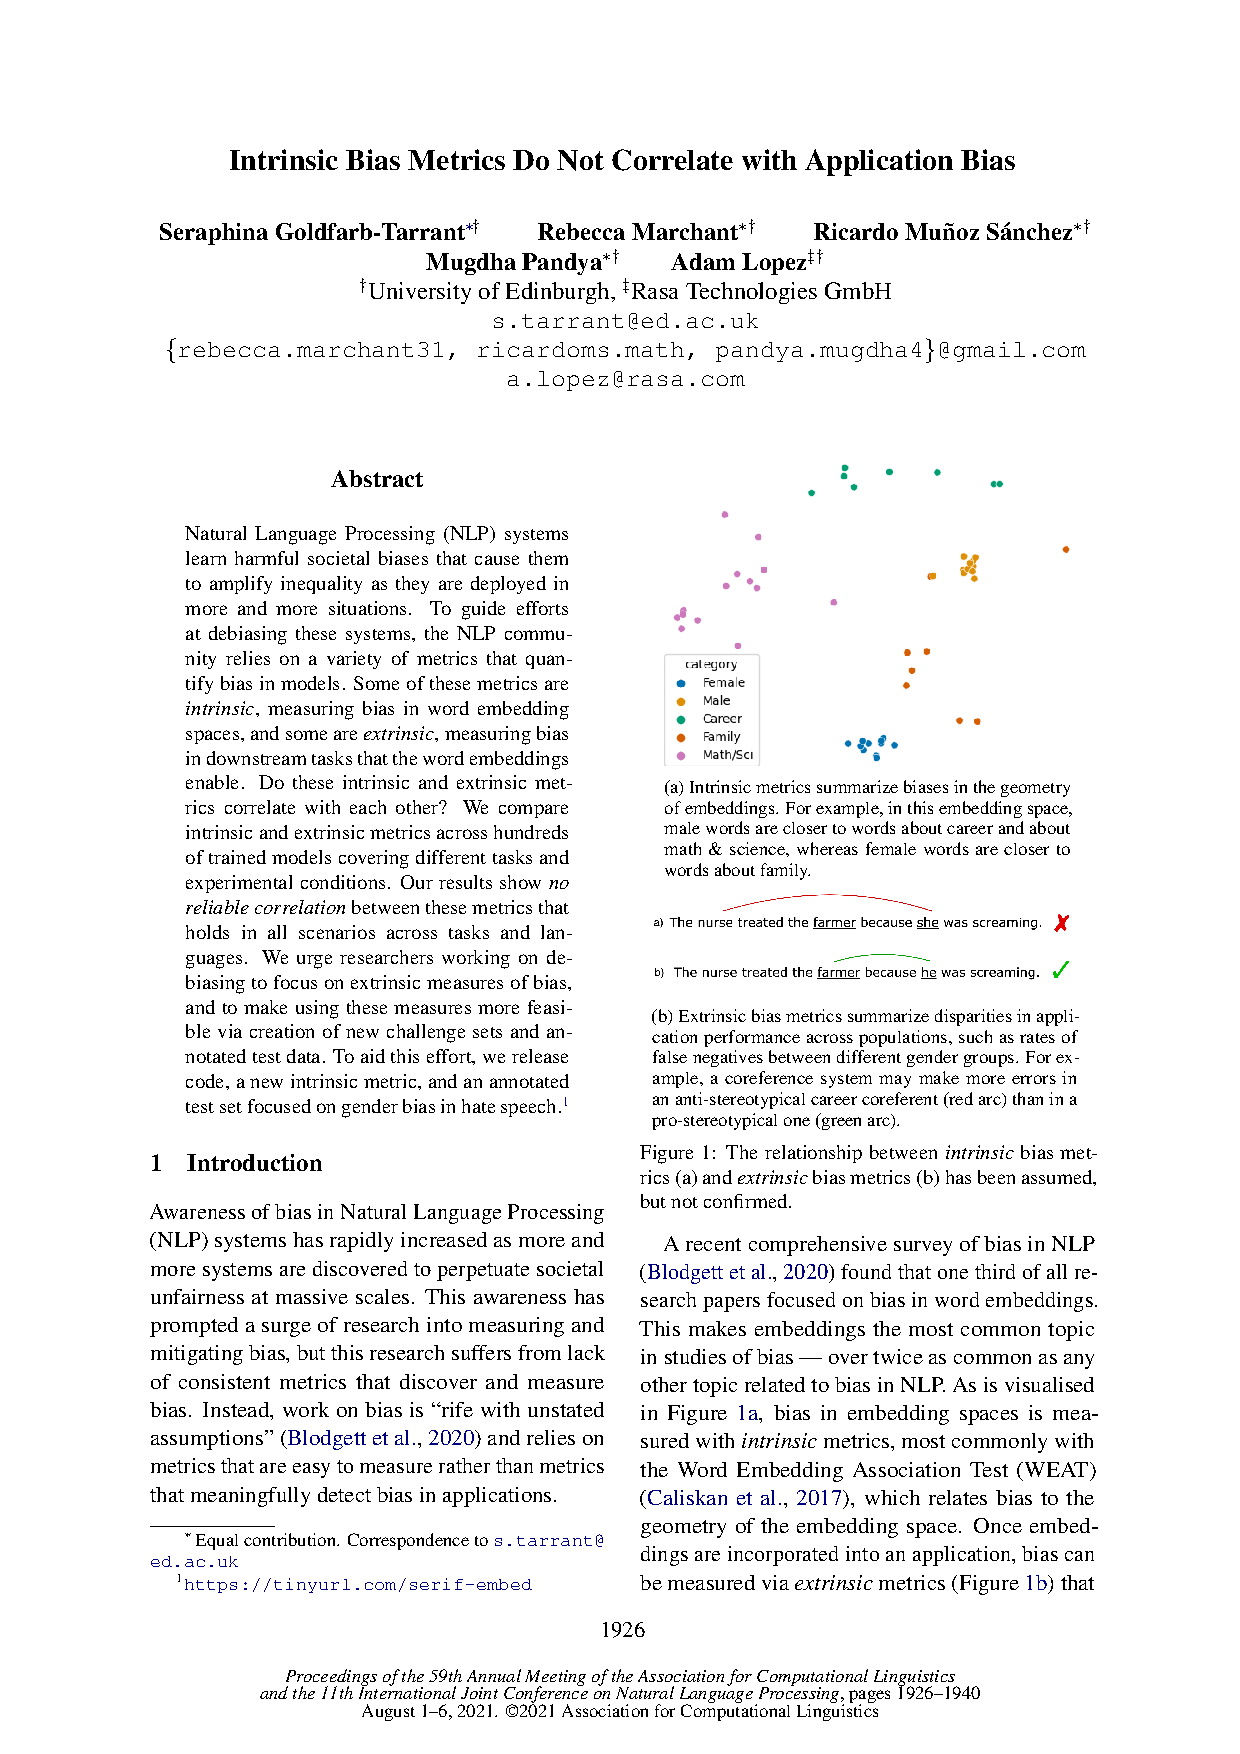
\includepdf[pages=-]{pdfs/2021.acl-long.150.pdf}

\chapter{How Gender Debiasing Affects Internal Model Representations,
and Why It Matters}\label{chapter:gender_bias_probing}


NEXT PICK UP HERE:
-motivated by previous work.
what is the best way to find a forward arrow of correlation, maybe to start backwards.




Notes:

Talk about how it extends to contextual (and concurrent work that finds the same thing)

Talk about the importance of multiple different metrics and maybe why (though I might not have the experiments to back this up).

Then also talk about what it means about transfer -- we can see what a language model will carry with it to something else. 


Can extend some sections and remove others if not doing by publication. Think about which ones to include.

Say which parts of the work I did since second author. 



Talk about probing as analysis: We can say that it is not a bias measurement but it is another method of analysis that we adapt into a bias measure.
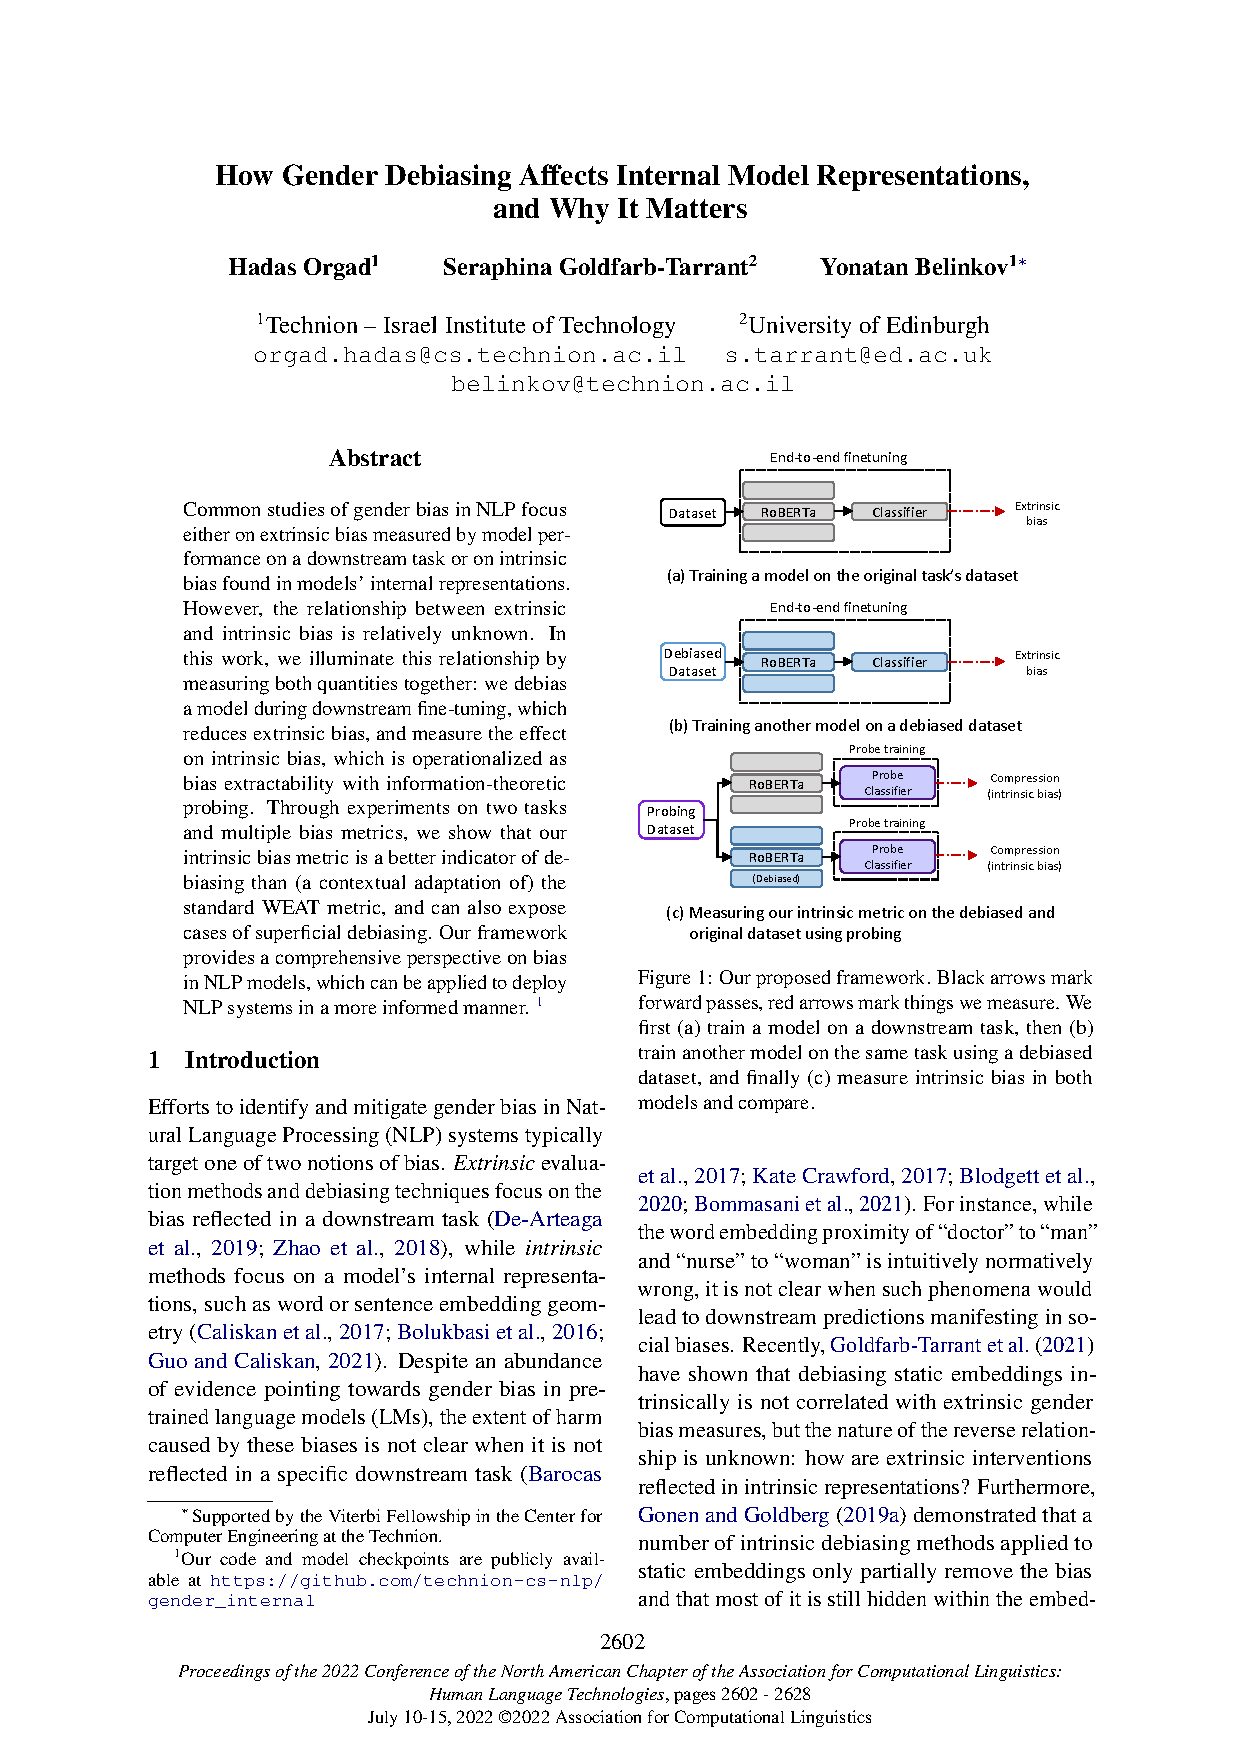
\includepdf[pages=-]{pdfs/2022.naacl-main.188.pdf}


\part{Fairness in Transfer across Languages}
\label{part:crosslingual}


Maybe consider adding label balance addendum
\chapter{A comparison of sentiment analysis with no transfer, monolingual transfer, and multilingual transfer}\label{chapter:x}

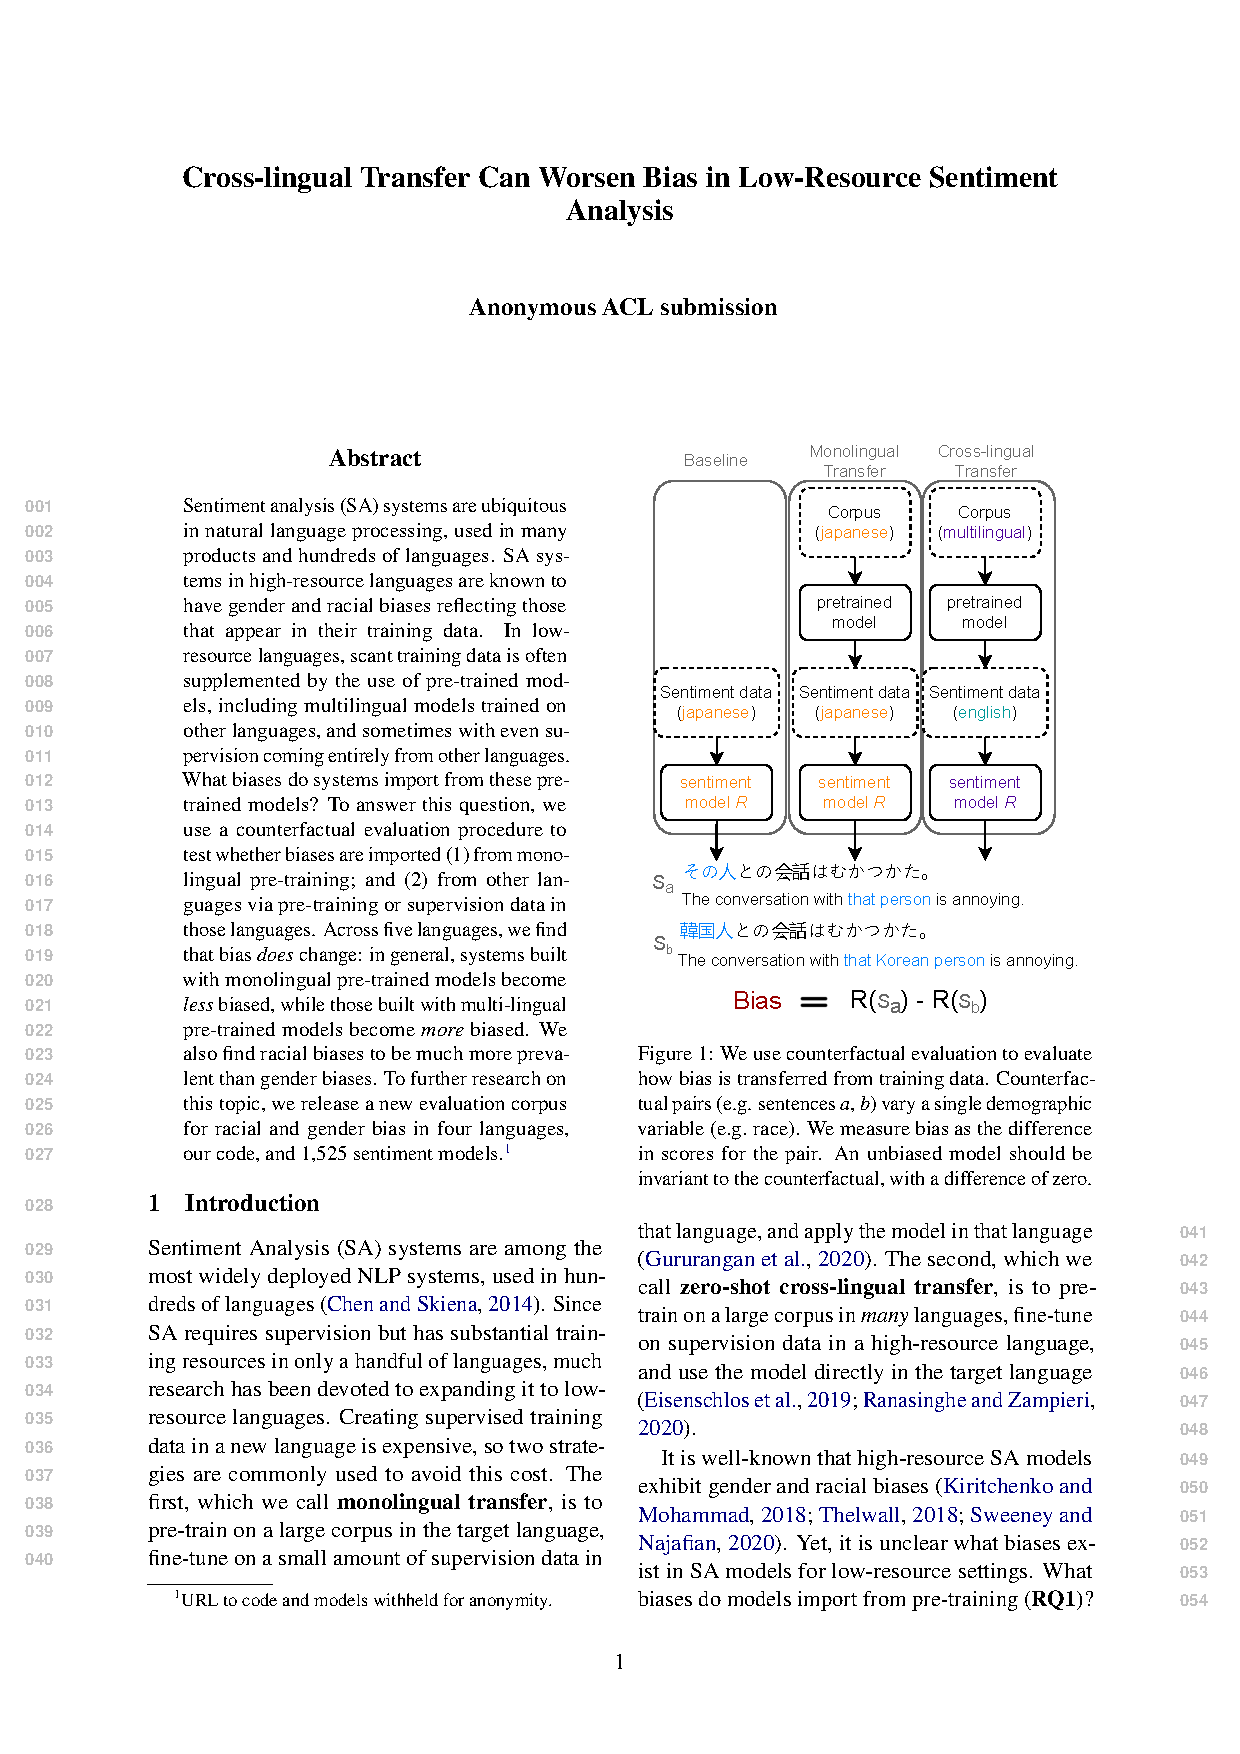
\includepdf[pages=-]{pdfs/sentiment_transfer_seraphina.pdf}

%\chapter{How does grammatical gender affect representations when it has no relationship to natural gender}\label{chapter:x}


\part{Generation and Causal intervention}\label{chapter:x}


\chapter{Conclusion}\label{chapter:conclusion}

%“For every subtle and complicated question, there is a perfectly simple and straightforward answer, which is wrong. —H.L. Mencken”
In this section I will condense the takeaways from my work, then expand them into the questions they pose. I'll discuss implications for future work, and do a bit more theorising than in each individual conclusion, made possible by the aggregation of all the works. I will also relate my work to the present day mania for Large Language models (LLMs), generative AI, and scaling.

This body of work has focused on \textbf{measurement of fairness}, and on then, with respect to those measurements, on \textbf{analysis of monolingual and cross-lingual transfer}, and analysis of \textbf{dense retrievers}. We contributing to enriching the understanding of fairness within a multi-part system, which was previously very poorly understood. This poverty was much more marked at the commencement of this work than today, but does still persist. Fairness and interpretability research have grown, but so has the field as a whole.\footnote{Fairness work has grown exponentially, but so have ACL and NeurIPS, both with about 40-50\% growth in submissions year over year, \url{https://aclweb.org/aclwiki/Conference_acceptance_rates} and \url{https://medium.com/criteo-engineering/neurips-2020-comprehensive-analysis-of-authors-organizations-and-countries-a1b55a08132e})} The scale and speed of productionisation still far outstrips understanding. 

In Part~\ref{part:measurement} I first examined the dominant method of bias evaluation in language models, based on embedding geometry and cosine similarity, found it to have poor predictive validity. I advocated for measuring bias downstream. 
I next found an alternative upstream measure in information theoretic probing of demographics. I caveat that it shows though only \textit{potential} for social bias downstream, a potential that may or may not be realised depending on classifier training. The full system is still needed to see the full picture.

In Part~\ref{part:crosslingual}, I examined monolingual and cross-lingual transfer in the setting of sentiment classification, in five languages, and found that both settings changed fairness outcomes. Monolingual transfer generally improved fairness despite the introduction of new data scraped from the depths of Common Crawl. I attributed this to increased stability in model decisions from the additional data: where stability is defined as not just less errors under the counterfactual, but smaller magnitude ones. Multilingual transfer, however, often worsened fairness outcomes, despite using more data than monolingual transfer. This may not contradict the previous result, as there are less parameters per language, such that even with regard to performance multilingual transfer models are not more stable than monolingual transfer models. The reasons for this difference are left to future work. 

In Part~\ref{part:generation}, I examined dense retrieval models, using the tools and research questions accumulated in Parts~\ref{part:measurement} and \ref{part:crosslingual}. I found that random initialisation and random data shuffle play a much larger role than previously thought. This challenges the standard practice of using only one random seed for research, which was then common and is now ubiquitous in the age of LLMs, where training one model takes over 400,000 kWh \citep{luccioni_bloom_carbon}, or the same amount of energy to make 14 million cups of tea, approximately the same amount that is drunk in Scotland daily.\footnote{It takes about 336000 joules to raise 1 liter (4 cups of tea) of water to a boil, which is equivalent to 0.116 kWh assuming an electric kettle at 80\% efficiency. This makes an LLM equivalent to approximately 13,714,286 cups of tea. The UK drinks on average 3 cups of tea per day, and the population of Scotland is 5.4 million today.} No one does this twenty five times, as I did here. In this work I also found a case where information theoretic probing was \textit{not} predictive of gender bias in retrievers, because the bias was caused by other factors beyond the model representation itself. 

The combined work in this thesis repeatedly shows how little it makes sense to make choices or come to conclusions about fairness without understanding and simulating the entire system. 

Each individual work raised as many questions as it answered, which have not yet been answered by other analytical work. These questions are significant in both size and importance and would be valuable extensions to the understanding of the field, even in the era of LLMs. For both works in Part~\ref{part:measurement} the question remains: what about generative models?  What is the relationship between upstream language model metrics and downstream bias in generation, as opposed to in classification? The objective in generation is more similar to that of pre-training, so the story may be different. Chapter~\ref{chapter:gender_bias_probing} showed that whether bias was realised was a property of both the language model and the classifier, so what if there's no classifier? 
But to answer that question, there has to be a way to measure bias in generation, which the field has by no means settled on, as we discuss in \S\ref{sec:measuring_fairness}. 

In Part~\ref{part:measurement} in classification, I used observational studies to determine allocational bias by measuring whether the error rates across populations that differ with respect to a demographic variable were equal (male group vs. female group, etc). In Part~\ref{part:crosslingual} I used interventional studies that measured whether change in a demographic variable changed predictions, when the predictions should be equal. Both of these measurements require a notion of equality -- which is very easy with a discrete label space or ordinal values. The same type of study could be set up for generative models: instead of classifying resumes, a model could write summaries of resumes with a recommendation to proceed or not, which is then read by a human.\footnote{This is what is happening in practice with generative AI now.} We can make the same assertion, that if we change the gender or race on the resume, the summary should not materially change. But what is a \textbf{material change}? In principle, it is a change that is large enough to cause the summary to be less accurate. Or to be equivalently accurate but to affect a human's opinion positively or negatively. Probably we want to know both for different reasons. How do we measure this? 

The little previous work on this raises just as many questions. \citet{vig_causal} consider social bias in generation to be the relative probability of different gendered pronouns along with stereotypical professions like \textit{doctor} and \textit{nurse}. But how would that be extended to different grammatical systems, like Turkish, which has no gendered pronouns? What about different demographic biases that aren't encoded the way gender is? There is far less research about those \citep{}, but they are no less important from the viewpoint of ethics or of law. 
%Even with those worked out, this measure is so zoomed in that, while it matters, it's hard to see what scope of bias problems it can and cannot represent. 
%BELOW IS REDUNDANT
%\citep{sheng-etal-2019} use \textit{regard} of the demographic that a generation is about, which is generalisable as a notion, but not in practice when operationalising: they train one classifier, which is available in English only, for three binaries (male/female, white/black, and gay/straight) and has never been updated. 
\citet{BOLD}, which is used in most LLM works today (e.g. \citep{llama2,jiang2024mixtral}) create a dataset where they use gender term frequency and regard, in combination with sentiment and toxicity, to try to overcome the issues of each. 
%Plenty of harmful stereotypes carry positive sentiment [example] and lots of social bias doesn't manifest via differences in toxicity [example. 
More essential measurement groundwork has to be done for generation before we can begin to determine whether these metrics are predictable from upstream metrics.

The second work in that section, Chapter~\ref{chapter:gender_bias_probing}, raises the question: what about beyond gender? Most work in this thesis by design looks as bias beyond gender (\ref{chapter:intrinsic_bias_metrics}, \ref{chapter:multilingual_sentiment_analysis}, and \ref{chapter:multilingual_sentiment_analysis_pt2} all include some notion of race or country of origin) but this one,  which proposes a new metric, looks only at gender (partly for lack of suitable datasets beyond it). But gender is encoded very differently in language than other demographic features, so it could reasonably have a different way it operates in model representations and social bias. In English, which weakly marks gender, and other languages with stronger gender agreement, gender is clearly important to represent for correct grammar and language reconstruction from a noising objective \citep{}. But race and country of origin are not as strong signals: it is not easy to determine these save from specific words like names (and even then the signal is not perfect at all, unlike with pronouns). How does this difference in encoded information affect the relationship between language models and downstream bias?

In Chapter~\ref{chapter:multilingual_sentiment_analysis} we found that there was less bias in aggregate in monolingual transfer, and more reasonable patterns of bias (less dramatic changes in sentiment score), but what about tracing individual examples through from pre-training? Could we track a specific negative stereotype in pre-training and see if it can affect decisions later? Extending to the work in Chapter~\ref{chapter:multilingual_sentiment_analysis_pt2}, could we extend tracing individual biases into multiple languages? Almost all bias research is done on aggregate information, and we extended our focus to be on patterns of bias, but we stopped short of doing fine-grained analysis. A more granular analysis would be valuable. We've spent this thesis tracing how fairness persists and travels through a system at a macro level, but we could extend this to a micro level. Such research would not even be bias specific; for there isn't concrete knowledge yet of how \textit{any} information travels between different training stages of models (of which there are increasingly many in the age of LLMs).

In Chapter~\ref{sec:fairness_as_other_fields}, I introduced the notion of fairness as a generalisation error vs. as a learnt dataset artifact (whether an artifact from spurious correlation or a historical bias). A deeper investigation into this could help enlighten why racial bias can increase with cross-lingual transfer. Is it really compounding biases (stereotypes) or could it be a generalisation error? One of these types of bias would have much less certainty than the other. Can an investigation into model uncertainty help illuminate which of these cases is involved in any measurements we observe?

Part~\ref{part:generation} shares the question of biases beyond gender from Chapter \ref{chapter:gender_bias_probing}, as it is also solely gender focused. It also raises many questions that have particular importance to fairness but are also general to our understanding of our systems as a whole. Why is random seed initialisation so important for bias and for generalisation? Why is it possible for a couple of seeds to \textit{just not work at all}, never mind fairness? Some of the anistropy of the representations from earlier training stages seems potentially predictive of later behaviour. Can we understand this well enough to utilise it? If so we could be able to actively encourage model training that is less prone to shortcutting. 

Now I want to bring this into current industry practice and zeitgeist. I do this partly because I've spent the better part of the last year working full-time on fairness at an LLM company. And partly because, in reviewing my PhD work, I don't want to ignore the sea change in NLP research that's taken place over the past year. I am not someone for whom `\textit{scaling is a way of life}'\footnote{This light shade given by Tatsunori Hashimoto when questioned about it at GenBench at EMNLP 2023.}, but it would be disingenuous, in a field intended to improve people's lives, to not speak about how my work relates to current research, current discourse, and current practice. This thesis was initially inspired by a sea change that I saw happening six years ago, after all. 

This work was all done on models three orders of magnitude smaller than the ones that I deal with in my work today. 

This does not matter at all. No conclusions in this thesis were model specific. If some architecture arises to replace neural embeddings, LSTMs, and Transformers which bears no genetic link to it, then they may no longer hold. But until that day (which will be very exciting, it would be nice to move on) the defferences between the models I use at work today and the models in this thesis are: 1) scale 2) a veneer of RLHF (Reinforcement Learning from Human Feedback \citep{} 3) instruction tuning \citep{} and 4) more math, logic, and code in both pretraining and fine-tuning than is usually present in NLP tasks (though some non-trivial amount will of course be present in CommonCrawl, which does drive the models in this thesis). None of these differences affect my conclusions. 

In my first rebuttal for \ref{chapter:intrinsic_bias_metrics}, temporally as well as sequentially the first paper in this thesis, Adam told me how to rebut one of the reviewers asking `But have you tried this on {\tt Newest Model Architecture}' (which in this case was BERT). He instructed me to turn that into a the question, `Is there any reason to expect that architecture would behave differently? Otherwise, they're just saying \textit{New thing is Magic}'. There is no reason to believe and of the four recent innovations change any of the discovered fairness behaviours here.

The replication and extension of my work in \ref{chapter:intrinsic_bias_metrics} by \citet{cao-etal-2022-intrinsic} did use BERT, and 18 other transformer architectures of varying sizes, and came to the same conclusions. 

We've seen the same bias amplification affects at scale \citep{} that we saw in \citet{zhao-etal-2017-men}. Current research shows that the RLHF (and family of alignment algorithms) predominantly affects style and structure of response, rather than content \citep{min-etal-2022-rethinking,  lin2023unlocking} and can be trivially changed and doesn't affect true fairness behaviour \citep{qi2023finetuning} and that all information is learnt at earlier stages, predominantly pretraining \citep{zhou2023lima}.
So the addition of an RLHF step to current SOTA models does not change any of these conclusions.

There is one salient change that will matter. Language models are essentially trained to compress and then reconstruct the data they were trained on, and this lossy compression has become less lossy as an effect of scaling \citep{karamolegkou-etal-2023-copyright}. This could change fairness outcomes, though will it help or will it harm? This depends somewhat on whether the source of the unfairness is a dataset artifact or a generalisation error (\S \ref{sec:fairness_as_other_fields}) in that overall increased memorisation is likely to exacerbate the learning of artifacts, but improve generalisation (though generalisation ability is difficult to test in the current era of closed language models and unknown pretraining and fine-tuning data). This effect from scaling won't change the measurements of mechanisms of bias transfer, which are the subject of this thesis, but they do lend weight to the need for more work on disentangling sources of bias and looking at the effects of increased memorisation from overparameterisation. 

When I started this thesis I focused on validating metrics, not because of a dedication to evaluation; I had grand plans for applying my ideas to cross-lingual bias mitigation. But I'd seen unvalidated assumptions in the standard metrics of the field, and it made me nervous about using those metrics in my own work. I didn't want to stake my PhD research and journey on a metric that I didn't believe in and find out 1.5 years in. But now that I work in a deployed product, I focus predominantly on evaluation. I do some fine-tuning and synthetic data creation, but about half my energy is spent on evaluation. Because good evaluation was \textit{always very hard} and the rise of generative AI has only made it harder. [do I need to say more here] And I can only throw darts at a wall if I know when they've hit something useful, and that's the hard part, not the dart throwing. 

There is some irony in how my first fairness work showed that you cannot do upstream social bias mitigation, and then I took a job where, to succeed, I am supposed to do just that. And where in practice, I need to, since education about NLP systems is not good enough that many of the people deploying language models have the knowledge or resources to do bias mitigation themselves. So, I use the tools and the ways of thinking and discoveries that I made over the course of this thesis to evaluate and analyse and create bounds for what types of bias could occur in different reasonable settings, and then make this information public, so that deployers know and can work around it. 

But this is still not satisfying enough. I do not think we will ever get to a point in which we rely on one single large pretrained model for thousands of use cases and can predict bias effects downstream for anything but the most common ones. All of this research has progressively taught me that I need to consider the entire NLP system in my measurements for bias: the pretraining, the fine-tuning, the task, the inputs, the corpus that a model can query. The limit case of this it that I need to consider the user interface, the users themselves, the societal power structures within which the NLP system is embedded. And I do think, at some stage, these do need to be part of the experiment conditions and considerations. We cannot consider the harmful effects of QA systems providing false information in absence of how it is displayed in a UI, and how much that UI encourages trust or overreliance \citep{} and bias research cannot consider stereotypes in absence of the power structures that make them harmful \citep{blodgett-etal-2021-stereotyping}. No more can most NLP systems be considered without these things, which all together make it increasingly challenging/impossible to predict all of these things at an upstream stage. 

But we can get to a point where we understand better what choices we've made in the lifecycle of an NLP system tend to make things worse or better, and why. With that, we can better predict bias potential in new systems and then with that knowledge set up evaluations and mitigation methods. So that we can take a set of facts about a model, and then generalise from it. %like humans do





% NOTES:
% The role of fairness research is the understanding that industry doesn't have time to do but that can still have hope of being applied in practice of having bearing on a real world situation -- this is a characteristic of the field since it is necessarily grounded in real humans and their lives.


%We are building out the picture of the full ecosystem of what can matter over the course of the thesis




% WHAT else can I bring in about science about goodharts law about things I've learnt about doing this all in practice?


%%% Outline what I want to cover in the discussion

\bibliographystyle{apalike}
\bibliography{anthology,bibl}

\appendix

\end{document}
